\documentclass[dvipdfmx]{beamer}

\usepackage{beamerthemesplit}
\usepackage[]{graphicx}
\graphicspath{%
{./slide08-img/}%
{./text08-img/}%
}

\usepackage{listings}
\usepackage{hyperref}
\usepackage{pxjahyper}
\usepackage{nameref} % これが\zexternaldocumentの前までに必要
\usepackage{zref-xr}
\usepackage{color}

\zxrsetup{toltxlabel} % 通常のLaTeXスタイルの\refを使う(\zexternaldocumentより前におく)
\zexternaldocument*[1:]{text08} % \zのついたexternaldocumentを使う

\setbeamertemplate{footline}[frame number]
\title{子どもIT未来塾 第8回}
\author{塾長 清水尚彦}

\def\quiz{1}

\begin{document}

\frame{
   \begin{center}
    \huge{子どもIT未来塾}\\

    \vspace{48pt}
	   \Large{第8回}\\
	   {\huge\bf スクレイピングを学ぼう}\\
    \vspace{24pt}
    \large{塾長 清水尚彦}\\
    \vspace{10pt}
    \large{\the\year 年 9月24日}
  \end{center}
}

\begin{frame}[fragile]
	\frametitle{今回の授業について ~~~\raisebox{-3mm}{
\includegraphics[width=0.1\textwidth]{raspberry}}}
		\begin{description}
			\item[目標] ~\\
				\begin{itemize}
					\item ウェブページから情報を取り出す方法(スクレイピング)について学ぼう
				\end{itemize}

			\item[授業の進め方]~\\
				\begin{itemize}
					\item 重要なことを先生が説明します
					\item スライドに示すページを開こう
					\item 例題・問題をすぐやろう\\
						やった問題にシールを貼ろう
				\end{itemize}
		\end{description}
		\vfill
		わからないことは、放っておかず、すぐにTAに聞きましょう
\end{frame}

\begin{frame}[fragile]
	\frametitle{スクレイピングを学ぼう:テキスト P.\pageref{1:P:intro}-P.\pageref{1:P:charCode}~~~\raisebox{-3mm}{
\includegraphics[width=0.1\textwidth]{raspberry}}}
  \large\textbf{友達の自己紹介ページをスクレイピングしてみよう}
        \begin{itemize}
            \item プログラムを使って、ウェブページから必要な情報だけを取りだすことをスクレイピングといいます。
        \end{itemize}
        \begin{minipage}{\textwidth}
            {\upshape
              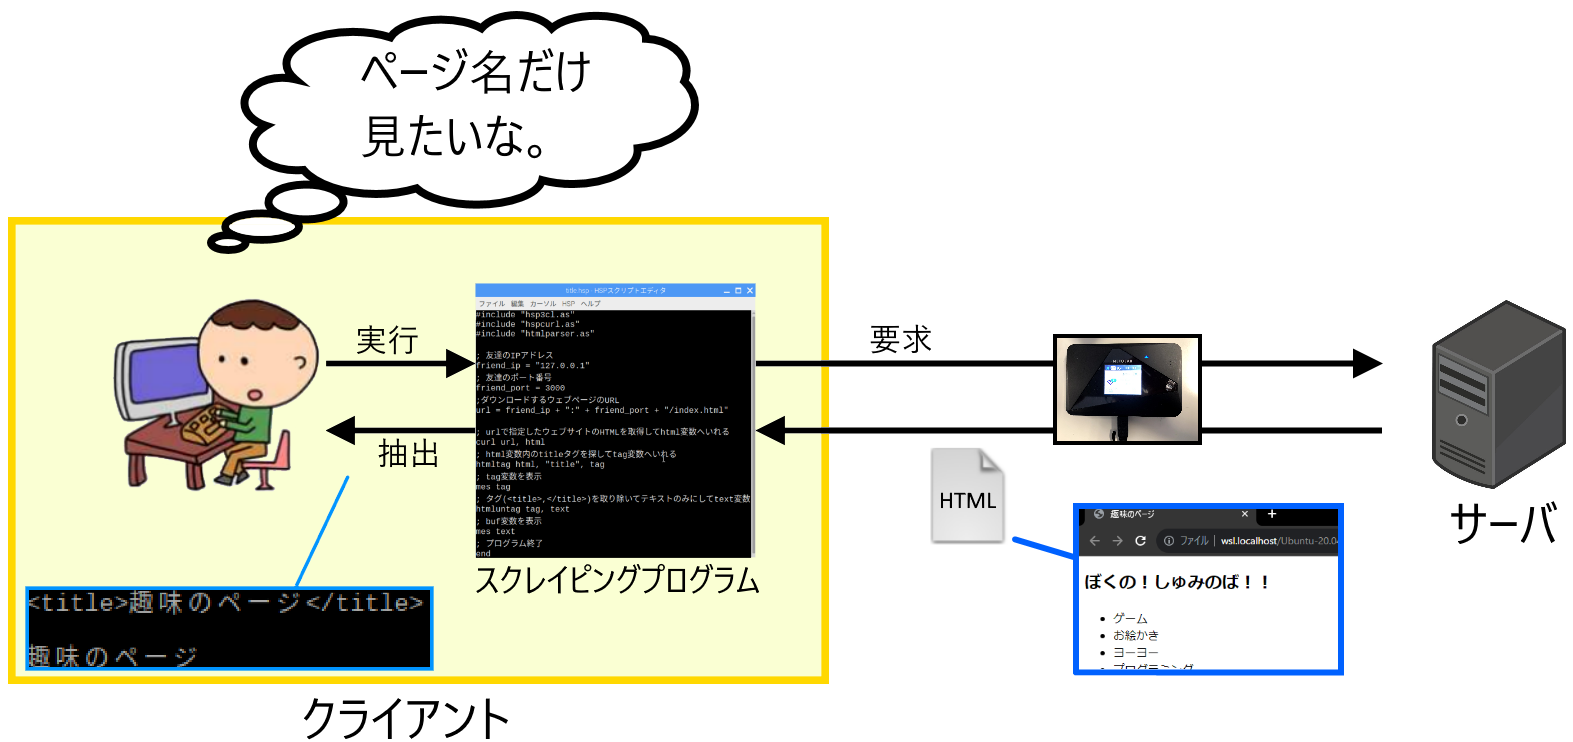
\includegraphics[width=\textwidth]{slide08-img003.png}}
        \end{minipage}
\end{frame}

\begin{frame}[fragile]
	\frametitle{スクレイピングを学ぼう:テキスト P.\pageref{1:P:intro}-P.\pageref{1:P:charCode}~~~\raisebox{-3mm}{
\includegraphics[width=0.1\textwidth]{raspberry}}}
        \begin{itemize}
            \item まず、第1回でつくった自己紹介ページと、ページで使っている画像をサーバプログラムがある場所にコピーしましょう。
        \end{itemize}
        \begin{minipage}{\textwidth}
            {\upshape
              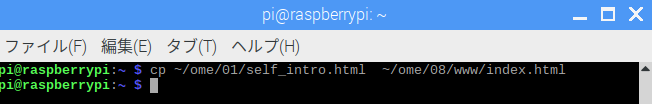
\includegraphics[width=\textwidth]{textbook-img002.png}}
        \end{minipage}
        \begin{itemize}
            \item 画像のコピーを忘れると、画像が表示されなくなります。
        \end{itemize}
        \begin{figure}
          \centering
          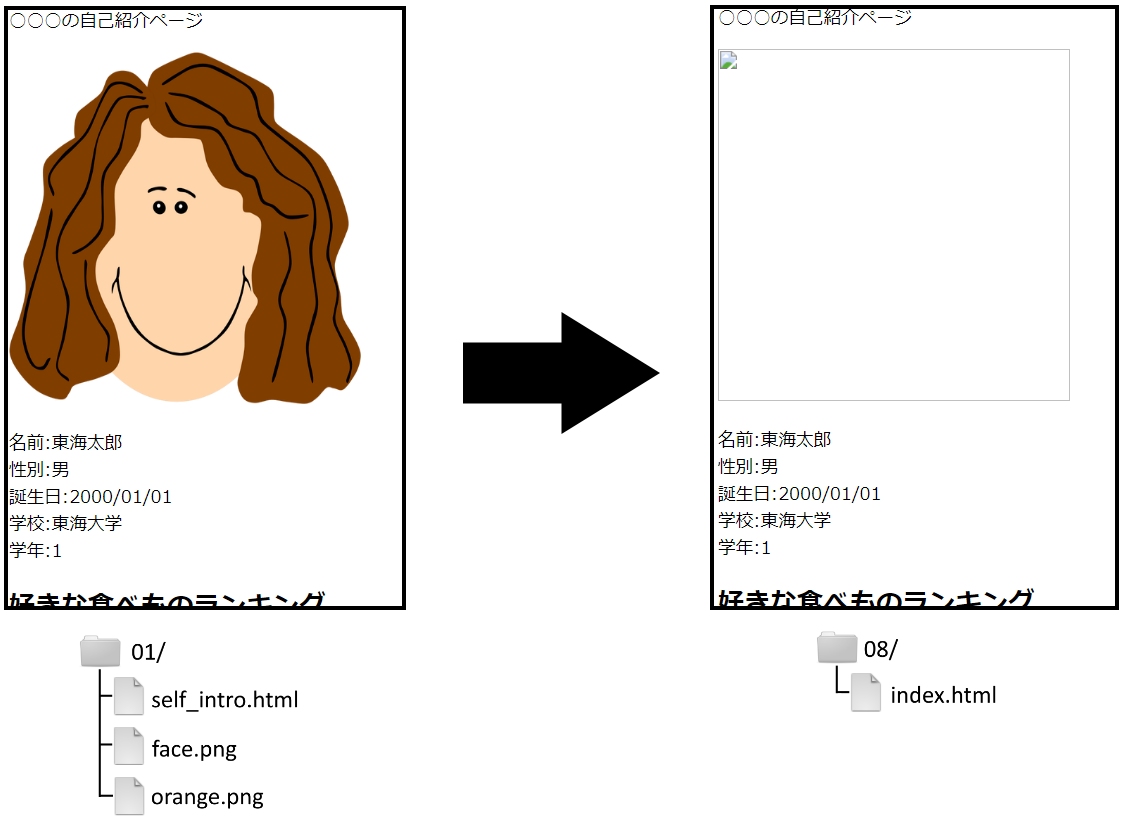
\includegraphics[width=0.65\textwidth]{slide08-img002.png}
        \end{figure}
\end{frame}

\begin{frame}[fragile]
	\frametitle{スクレイピングを学ぼう:テキスト P.\pageref{1:P:intro}-P.\pageref{1:P:charCode}~~~\raisebox{-3mm}{
\includegraphics[width=0.1\textwidth]{raspberry}}}
        \begin{itemize}
            \item グループの友達とIPアドレスを教え合いましょう。教科書P.xのIPアドレスメモ欄にメモしておきましょう。
        \end{itemize}
        \begin{minipage}{\textwidth}
            {\upshape
              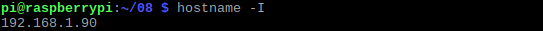
\includegraphics[width=\textwidth]{slide08-img001.png}}
        \end{minipage}
        \begin{itemize}
            \item 終わったら、ウェブサーバを立ち上げましょう。
        \end{itemize}
        \begin{minipage}{\textwidth}
            {\upshape
              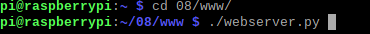
\includegraphics[width=\textwidth]{textbook-img003.png}}
        \end{minipage}
\end{frame}

\begin{frame}[fragile]
	\frametitle{スクレイピングを学ぼう:テキスト P.\pageref{1:P:intro}-P.\pageref{1:P:charCode}~~~\raisebox{-3mm}{
\includegraphics[width=0.1\textwidth]{raspberry}}}
      \large\textbf{教科書をよみながら、例題をやってみよう}
				\begin{itemize}
					\item \ref*{1:E:CURL}
					\item \ref*{1:E:HTML}
					\item \ref*{1:E:SCRAPING}
				\end{itemize}
      \vfill
      \large\textbf{速く終わった子は、次の問題をやってみよう}
				\begin{itemize}
					\item \ref*{1:Q:CURL}, \ref*{1:Q:HTML}
					\item \ref*{1:Q:title}, \ref*{1:Q:mes}, \ref*{1:Q:ol}, \ref*{1:Q:tag}
				\end{itemize}
      \vfill
      \large\textbf{わからないことは、放っておかず、すぐに TA に聞きましょう}
\end{frame}

\end{document}
